% Also note that the "draftcls" or "draftclsnofoot", not "draft", option
% should be used if it is desired that the figures are to be displayed in
% draft mode.
%

\setlength{\paperheight}{11in}
\setlength{\paperwidth}{8.5in}

%\documentclass[conference]{IEEEtran}
%\documentclass{acm_proc_article-sp}
\documentclass{sig-alternate}

% correct bad hyphenation here
\hyphenation{op-tical net-works semi-conduc-tor}

% Optionally save space in lists (place this command after a list environment (e.g., itemize, enumerate, description)
\newcommand{\compresslist}{
	\vspace{-.5em}
	\setlength{\itemsep}{1pt}
	\setlength{\parskip}{0pt}
	\setlength{\parsep}{0pt}
}

\usepackage{flushend}

\usepackage{listings}
\usepackage{subfigure}
\usepackage{cite}
\usepackage{url}
\usepackage{tabularx}
\usepackage[table, svgnames]{xcolor} 
\usepackage{color}
\usepackage{siunitx}
\usepackage{multirow}
\usepackage{wasysym}
\usepackage{times}
\usepackage{graphicx}
\usepackage{epsf}
\usepackage{verbatim}
\usepackage{psfig}
\usepackage{cite}
\usepackage{url}
\usepackage{color}
\usepackage[table]{xcolor}
\usepackage{booktabs, dcolumn}
\usepackage{alltt}

\usepackage{longtable,lscape}
\usepackage{slashbox,multirow}
\usepackage{colortbl}
\usepackage{mathrsfs}

\newcommand{\Add}{\CodeIn{add}}
\newcommand{\AVTree}{\CodeIn{AVTree}}
\newcommand{\Assignment}[3]{$\langle$ \Object{#1}, \Object{#2}, \Object{#3} $\rangle$}
\newcommand{\BinaryTreeRemove}{\CodeIn{BinaryTree\_remove}}
\newcommand{\BinaryTree}{\CodeIn{BinaryTree}}
\newcommand{\Caption}{\caption}
\newcommand{\Char}[1]{`#1'}
\newcommand{\CheckRep}{\CodeIn{checkRep}}
\newcommand{\ClassC}{\CodeIn{C}}
\newcommand{\CodeIn}[1]{{\small\texttt{#1}}}
\newcommand{\CodeOutSize}{\scriptsize}
\newcommand{\Comment}[1]{}
\newcommand{\Ensures}{\CodeIn{ensures}}
\newcommand{\ExtractMax}{\CodeIn{extractMax}}
\newcommand{\FAL}{field-ordering}
\newcommand{\FALs}{field-orderings}
\newcommand{\Fact}{observation}
\newcommand{\Get}{\CodeIn{get}}
\newcommand{\HashSet}{\CodeIn{HashSet}}
\newcommand{\HeapArray}{\CodeIn{HeapArray}}
\newcommand{\Intro}[1]{\emph{#1}}
\newcommand{\Invariant}{\CodeIn{invariant}}
\newcommand{\JUC}{\CodeIn{java.\-util.\-Collections}}
\newcommand{\JUS}{\CodeIn{java.\-util.\-Set}}
\newcommand{\JUTM}{\CodeIn{java.\-util.\-TreeMap}}
\newcommand{\JUTS}{\CodeIn{java.\-util.\-TreeSet}}
\newcommand{\JUV}{\CodeIn{java.\-util.\-Vector}}
\newcommand{\JMLPlusJUnit}{JML+JUnit}
\newcommand{\Korat}{Korat}
\newcommand{\Left}{\CodeIn{left}}
\newcommand{\Lookup}{\CodeIn{lookup}}
\newcommand{\MethM}{\CodeIn{m}}
\newcommand{\Node}[1]{\CodeIn{N}$_#1$}
\newcommand{\Null}{\CodeIn{null}}
\newcommand{\Object}[1]{\CodeIn{o}\ensuremath{_#1}}
\newcommand{\PostM}{\MethM$_{post}$}
\newcommand{\PreM}{\MethM$_{pre}$}
\newcommand{\Put}{\CodeIn{put}}
\newcommand{\Remove}{\CodeIn{remove}}
\newcommand{\RepOk}{\CodeIn{repOk}}
\newcommand{\Requires}{\CodeIn{requires}}
\newcommand{\Reverse}{\CodeIn{reverse}}
\newcommand{\Right}{\CodeIn{right}}
\newcommand{\Root}{\CodeIn{root}}
\newcommand{\Set}{\CodeIn{set}}
\newcommand{\State}[1]{2^{#1}}
\newcommand{\TestEra}{TestEra}
\newcommand{\TreeMap}{\CodeIn{TreeMap}}

\newenvironment{CodeOut}{\begin{scriptsize}}{\end{scriptsize}}
\newenvironment{SmallOut}{\begin{small}}{\end{small}}

\newcommand{\pairwiseEquals}{PairwiseEquals}
\newcommand{\monitorEquals}{MonitorEquals}
%\newcommand{\monitorWField}{WholeStateW}
\newcommand{\traverseField}{WholeState}
\newcommand{\monitorSMSeq}{ModifyingSeq}
\newcommand{\monitorSeq}{WholeSeq}

\newcommand{\IntStack}{\CodeIn{IntStack}}
\newcommand{\UBStack}{\CodeIn{UBStack}}
\newcommand{\BSet}{\CodeIn{BSet}}
\newcommand{\BBag}{\CodeIn{BBag}}
\newcommand{\ShoppingCart}{\CodeIn{ShoppingCart}}
\newcommand{\BankAccount}{\CodeIn{BankAccount}}
\newcommand{\BinarySearchTree}{\CodeIn{BinarySearchTree}}
\newcommand{\LinkedList}{\CodeIn{LinkedList}}

\newcommand{\Book}{\CodeIn{Book}}
\newcommand{\Library}{\CodeIn{Library}}

\newcommand{\Jtest}{Jtest}
\newcommand{\JCrasher}{JCrasher}
\newcommand{\Daikon}{Daikon}
\newcommand{\JUnit}{JUnit}

\newcommand{\trie}{trie}

\newcommand{\Perl}{Perl}


\newcommand{\SubjectCount}{11}
\newcommand{\DSSubjectCount}{two}

\newcommand{\Equals}{\CodeIn{equals}}
\newcommand{\Pairwise}{PairwiseEquals}
\newcommand{\Subgraph}{MonitorEquals}
\newcommand{\Concrete}{WholeState}
\newcommand{\ModSeq}{ModifyingSeq}
\newcommand{\Seq}{WholeSeq}
\newcommand{\Aeq}{equality}

\newcommand{\Meaning}[1]{\ensuremath{[\![}#1\ensuremath{]\!]}}
\newcommand{\Pair}[2]{\ensuremath{\langle #1, #2 \rangle}}
\newcommand{\Triple}[3]{\ensuremath{\langle #1, #2, #3 \rangle}}
\newcommand{\SetSuch}[2]{\ensuremath{\{ #1 | #2 \}}}

\newcommand{\Equiv}[2]{\ensuremath{#1 \EquivSTRel{} #2}}
\newcommand{\EquivME}{\Equiv}
\newcommand{\EquivST}{\Equiv}
\newcommand{\EquivSTRel}{\ensuremath{\cong}}
\newcommand{\Redundant}[2]{\ensuremath{#1 \lhd #2}}
\newcommand{\VB}{\ensuremath{\mid}}
\newcommand{\MES}{method-entry state}

\newcommand{\Small}[1]{{\small{#1}}}

\newcommand{\CenterCell}[1]{\multicolumn{1}{c|}{#1}}

% Yoonki's code
\colorlet{tableheadcolor}{gray!25} % Table header colour = 25% gray
\newcommand{\headcol}{\rowcolor{tableheadcolor}} %
\colorlet{tablerowcolor}{gray!10} % Table row separator colour = 10% gray
\newcommand{\rowcol}{\rowcolor{tablerowcolor}} %
    % Command \topline consists of a (slightly modified) \toprule followed by a \heavyrule rule of colour tableheadcolor (hence, 2 separate rules)
\newcommand{\topline}{\arrayrulecolor{black}\specialrule{0.1em}{\abovetopsep}{0pt}%
            \arrayrulecolor{tableheadcolor}\specialrule{\belowrulesep}{0pt}{0pt}%
            \arrayrulecolor{black}}
    % Command \midline consists of 3 rules (top colour tableheadcolor, middle colour black, bottom colour white)
\newcommand{\midline}{\arrayrulecolor{tableheadcolor}\specialrule{\aboverulesep}{0pt}{0pt}%
            \arrayrulecolor{black}\specialrule{\lightrulewidth}{0pt}{0pt}%
            \arrayrulecolor{white}\specialrule{\belowrulesep}{0pt}{0pt}%
            \arrayrulecolor{black}}
    % Command \rowmidlinecw consists of 3 rules (top colour tablerowcolor, middle colour black, bottom colour white)
\newcommand{\rowmidlinecw}{\arrayrulecolor{tablerowcolor}\specialrule{\aboverulesep}{0pt}{0pt}%
            \arrayrulecolor{black}\specialrule{\lightrulewidth}{0pt}{0pt}%
            \arrayrulecolor{white}\specialrule{\belowrulesep}{0pt}{0pt}%
            \arrayrulecolor{black}}
    % Command \rowmidlinewc consists of 3 rules (top colour white, middle colour black, bottom colour tablerowcolor)
\newcommand{\rowmidlinewc}{\arrayrulecolor{white}\specialrule{\aboverulesep}{0pt}{0pt}%
            \arrayrulecolor{black}\specialrule{\lightrulewidth}{0pt}{0pt}%
            \arrayrulecolor{tablerowcolor}\specialrule{\belowrulesep}{0pt}{0pt}%
            \arrayrulecolor{black}}
    % Command \rowmidlinew consists of 1 white rule
\newcommand{\rowmidlinew}{\arrayrulecolor{white}\specialrule{\aboverulesep}{0pt}{0pt}%
            \arrayrulecolor{black}}
    % Command \rowmidlinec consists of 1 tablerowcolor rule
\newcommand{\rowmidlinec}{\arrayrulecolor{tablerowcolor}\specialrule{\aboverulesep}{0pt}{0pt}%
            \arrayrulecolor{black}}
    % Command \bottomline consists of 2 rules (top colour
\newcommand{\bottomline}{\arrayrulecolor{white}\specialrule{\aboverulesep}{0pt}{0pt}%
            \arrayrulecolor{black}\specialrule{\heavyrulewidth}{0pt}{\belowbottomsep}}%
\newcommand{\bottomlinec}{\arrayrulecolor{tablerowcolor}\specialrule{\aboverulesep}{0pt}{0pt}%
            \arrayrulecolor{black}\specialrule{\heavyrulewidth}{0pt}{\belowbottomsep}}%

\usepackage{dcolumn}
\newcolumntype{Y}{D..{6.4}}

%\newcommand{\blind}[1]{{\color{white}\{#1\}}}
\newcommand{\blind}[1]{#1}

\clubpenalty = 10000
\widowpenalty = 10000
\displaywidowpenalty = 10000

%
% paper title
% can use linebreaks \\ within to get better formatting as desired
% Do not put math or special symbols in the title.
\begin{document}
\toappear{}
%Strategic analysis of static analysis defect resolution
%Analyzing, supporting?
%Straticheck: Identifying Successful Strategies for Resolving IDE Notifications
%Helping developers uses\ successful strategies to resolve static analysis notifications
\title{Identifying Successful Strategies for Resolving Static Analysis Notifications}

\numberofauthors{1}
\author{
\alignauthor Justin Smith\\
\affaddr{North Carolina State University}\\
\affaddr{Raleigh, NC, USA} \\
\email{jssmit11@ncsu.edu}
}

\maketitle


\begin{abstract}
Static analysis tools have increasingly drawn attention from the research community because they afford the early detection of potential code defects.
Unfortunately, static analysis tools do not fully support developers in resolving the defects they detect.
Instead, developers must rely on their own knowledge of good defect resolution \textit{strategies}.
Accurately and efficiently resolving defects is a complex task that often requires considerable effort from developers.
For example, some defects require developers to forage for additional information, determine whether the defect is a false positive, use code navigation and debugging tools, consult team members, and modify the source code. 
In this work I perform a preliminary analysis of the successful and unsuccessful strategies developers use to resolve these defects and outline a tool that, based on the successful strategies I identified, supports developers throughout the defect resolution process. 


\end{abstract}

% % A category with the (minimum) three required fields
% \category{H.4}{Information Systems Applications}{Miscellaneous}
% %A category including the fourth, optional field follows...
%\category{D.2.6}{Software Engineering}{Programming Environments}
%\keywords{XXXXX}

\section{Introduction}
\label{sec:intro}
Static analysis tools help developers locate various code defects early in the development process, even before the code executes. 
For example, static analysis tools detect access control vulnerabilities~\cite{Aside}, potential null dereferences~\cite{FindBugs}, and concurrency bugs~\cite{ThreadSafe} by analyzing source code.
Detecting, and more importantly, resolving defects like these early can prevent more costly failures later in the development process~\cite{ayewah2008using}.

In their defect reports, static analysis tools provide information to developers in the form of textual \textit{notifications}.
These notifications typically describe possible defects.
However, they often fail to fully support developers in actually resolving the defects they detect~\cite{Johnson2013}.
For example, accurately resolving defects can require developers to identify false positives, explore the existing code, invoke additional tools, modify the code, and verify the correctness of their fix, among other activities~\cite{Smith2015}.  
Even with notifications that afford actionable ``Quick Fix'' suggestions, developers must still determine whether those suggestions are appropriate for their code.
Consider one of the most common \cite{Ayewah2007} notifications produced by FindBugs, a static analysis tool, which in this case, does not provide any imperative suggestions:

%\begin{lstlisting}[language=Java, keywordstyle=\color{blue}]
%object.add("foo");
%if (object != null){
% object.add("foo");
%}
%\end{lstlisting}

\vspace{2mm}

\begin{tabular}{|p{7.5cm}}
	``There is a branch of statement that, if executed, guarantees that a null value will be dereferenced, which would generate a NullPointerException when the code is executed. Of course, the problem might be that the branch or statement is infeasible and that the null pointer exception can't ever be executed; \textbf{deciding that is beyond the ability of FindBugs.}"\\
\end{tabular}
\vspace{2mm}

\noindent
The notification clearly identifies the problem with the code (a null value may be dereferenced), however the notification provides no suggestions about how the developer should proceed to resolve the defect. 
The actions developers take to resolve defects, I refer to collectively as the developer's defect resolution \textit{strategy}.
For example, one strategy for resolving this defect, which decomposes into three sub-strategies, would be to use Google to search for information about NullPointerExceptions, use Eclipse's call hierarchy tool to explore which branches get executed, and finally add an additional null check only if deemed appropriate.
Of course, there exist other strategies for resolving this defect.

I envision an alternative paradigm in which static analysis tool notifications explicitly support the resolution of the defects they detect by orchestrating the actions developers take and tools developers use.
In this paper, I contribute: 

\begin{enumerate}
	\compresslist
	\item A preliminary analysis of the successful and unsuccessful strategies developers use to resolve defects detected by static analysis, and
	\item A description of a tool that explicitly provides developers with successful defect resolution strategies.
	
\end{enumerate}

%Why should tools do this? They have privileged information about the defect. Already computed information about the relevant areas in the code. 

%When interacting with a given static analysis notification, a developer's current task is well known. I can leverage that knowledge to provide context sensitive information about effective strategies.

\section{Related Work}
\label{sec:rw}
%In this section, I briefly survey related work.
%\subsection{Defect Resolution}
Several researchers have stressed the importance of supporting defect resolution.
For example, Path Projection~\cite{Khoo2008} facilitates defect resolution by presenting program path visualizations. 
Quick Fix Scout~\cite{Muslu2012} also supports defect resolution, in this case by performing speculative analysis and therefore enabling developers to preview and compare fixes.
Taken alone, Path Projection and Quick Fix Scout each only support one step in the defect resolution process.
In contrast, I am working toward supporting developers throughout every step of the defect resolution process.

%\subsection{Supporting Effective Strategies}
Previous research has also focused on the importance of supporting successful strategies in the use of complex computer applications.
In computer-aided design applications, for example, Bhavnani and John have measured the performance costs of inefficient strategies~\cite{Bhavnani2000}.
Their results suggest the use of more efficient strategies leads to faster task completion time and more accurate results.
They also show that offline educational interventions can increase the use of efficient strategies.
Leaning on the work of Bhavnani and John, Cockburn and colleagues review interface research and state that knowledge of efficient strategies is also an important factor influencing the novice to expert transition~\cite{Cockburn2014}.
In his work, Cockburn discusses several techniques for designing interfaces that implicitly encourage the use of efficient strategies.
These research efforts emphasize the importance of educating users about efficient strategies, however neither proposes to do so by explicitly prescribing effective strategies to users while they complete the relevant task.
Building off this previous work, my approach aims to proliferate strategic knowledge by explicitly describing successful strategies. 

%rather than designing systems that implicitly encourage them.

%In resloving defects this is feasible, because the specific task is know a priori


%In other disciplines, the explanation of successful strategies is critical to the accurate completion of tasks. In the natural sciences, lab protocols are written guidelines that describe strategies for successfully completing an experiment. Recently, Abbott and colleagues examined the parallels between lab protocols and mixed initiative systems [Cite VL/HCC paper]. 

%For example, in the culinary arts recipes capture all of the strategic information needed to complete cooking tasks~\cite{Recipes2013}.



 %Brittany's stuff, my stuff
 
 
 %Unlike complex applications that Bhavnani and John studied, 



\section{Approach}
\label{sec:approach}
%\subsection{Analyze existing notifications for strategy support?}
%Debating adding another section here, but will want to discuss in reading group.
%Analyze all FB messages to determine to what extent static analysis notifications support holistic fixes
%how actionable?
%Only X\% of FindBugs notifications include information about how to resolve the defect. 

%
To enable tools to support developers in executing accurate and efficient strategies, I must first identify which strategies are successful. 
I have already conducted a study~\cite{Smith2015} in which I recorded ten developers resolving four security defects while using Find Security Bugs (FSB)~\cite{FindSecurityBugs} --- a security-oriented extension of FindBugs~\cite{FindBugs}.
Extending my previous work, in this work I reanalyzed the audio and video recordings from~\cite{Smith2015}, focusing on identifying those successful and unsuccessful strategies developers used to resolve the defects FSB detected.

Returning to the example of a defect resolution strategy from Section~\ref{sec:intro}, Figure~\ref{fig:description} depicts the notation I used to represent defect resolution strategies. 
Similar to the notion of attack trees~\cite{attackTrees}, which hierarchically organize the actions an attacker could take to exploit a system, this hierarchical representation, which I will refer to as a \textit{strategy tree}, describes defect resolution strategies as a structured sets of actions.
Recursively, each child of the root is itself a strategy tree representing the sub-strategies developers used.
Finally, to measure success granularly, I annotated a sub-strategy in the tree whenever it either contributed to or detracted from the accurate resolution of the defect --- green and red lines prefixed with $+$/$-$, respectively.


\begin{figure}
	\centering
	\includegraphics[width=\columnwidth]{"images/strategy description format"}
	\caption{Example strategy tree for the null dereference defect. }
	\label{fig:description} 

\end{figure}


%\subsection{Supplementing Observed Strategies}

%Since the developers I observed range in experience levels and may not have executed all of the most successful strategies, I supplement the observed strategies by examining defect resolution strategies published by trusted authorities. In particular, I incorporated information published by OWASP and the CVE.

%



\section{Results}
Because different developers might use different strategies to resolve the same defect, I constructed 40 strategy trees --- one for each top-level strategy I observed in the study. With an average branching factor of approximately four at the roots, these 40 top-level strategies decompose into 155 sub-strategies. 

I inspected the strategies for similarity to determine the feasibility of recommending strategies that apply more broadly.
The strategies I observed vary depending on the individual developer.
For example, the three developers who reported the least familiarity with security vulnerabilities started 11 of the 12 tasks by reading the notification text.
In contrast, more experienced developers started by reading the code.
The two developers who reported the highest familiarity with security vulnerabilities started only 2 of 8 tasks by reading the notification text. 

Though all the strategies I identified exhibit slight differences (such as how developers chose to start resolving the defect), promisingly, some common patterns emerged across participants and defects. 
In all 40 strategies, developers read the code surrounding the defect. Furthermore, in 90\% of the strategies developers read the notification text and in 75\% of the strategies developers tried to determine if the notification was a false positive.

%Inexperience read the notification. Promising for our intervention

%At least given a defect?
%Some underlying patterns possible to suggest strategies that apply generally
%Promising, because it may suggest the possibility of sharing strategies across developers.

Examining the strategies based on the degree to which they lead to successful outcomes, I observed 62 strategic failures (i.e, instances where a developer's strategy was not efficient or accurate).
For example, one developer used Eclipse's call hierarchy tool attempting to locate all the call locations of a \CodeIn{doPost()} method. The tool located several explicit call locations within test classes. However, it did not locate implicit calls that originated from HTML pages.
This lead the developer to incorrectly conclude that the code was safe, because users did not have access to the vulnerable method. 
I observed at least one strategic failure in 27 of 40 tasks; across the four tasks, every developer's strategies were undermined by at least one failure.
The prevalence of strategic failures, even among the the most experienced developers I studied, further motivates this work.

Despite the lack of tool support, some developers resolved some defects correctly using successful strategies. I observed 105 instances where developers' defect resolution strategies succeeded in leading them to make observable progress on the resolution task.

Drawing from the successful strategies I observed, I sketched (Figure~\ref{fig:tool}) a tool that presents explicit defect resolution strategies to developers. 
The strategy this tool presents is a composite strategy, combining the ten strategies I observed developers using for one task.
Since the developers I studied may not have executed all of the most successful strategies, I supplement the tool by also including defect resolution recommendations published by trusted authorities such as OWASP and CVE~\cite{OWASP, CVE}.
The tool also includes checkboxes to allow developers to track their progress.
Additionally, the tool exposes other tools (Open Declaration in this example) in contexts when they would be most helpful.

\begin{figure}
	\centering
	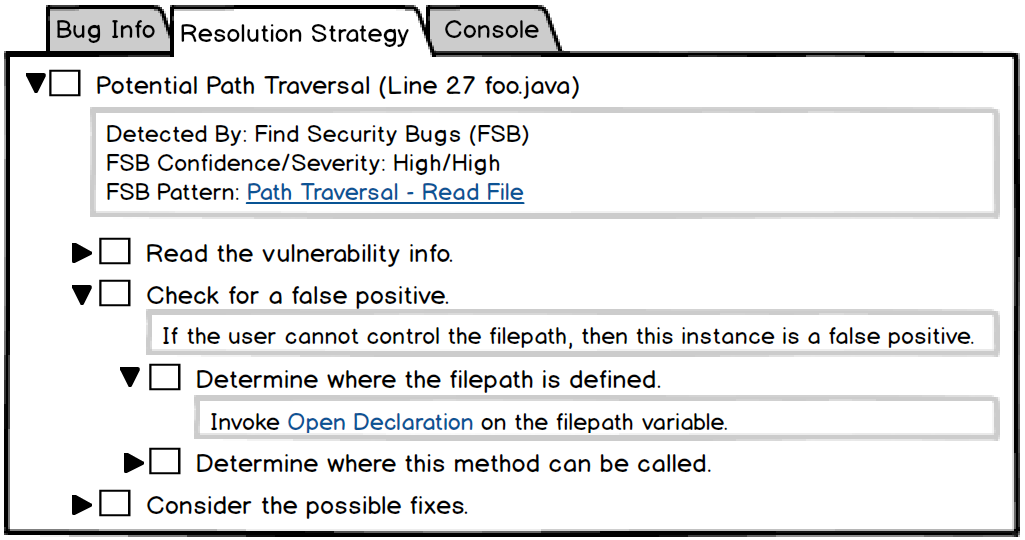
\includegraphics[width=\columnwidth]{images/toolscreenshot}
	\caption{A mockup of a tool that presents successful strategies.}
	\label{fig:tool} 
\end{figure}



\section{Contributions}
%
My preliminary analysis of developers' strategies suggests that strategic failures may undermine developers' in accurately and efficiently resolving defects.  
I propose a new tool that helps developers resolve defects by providing them with explicit descriptions of successful strategies.
Used in practice, such an approach may improve code quality and also educate developers by increasing their awareness of more successful strategies.

%work I present a tool, Strategy-Check, that embraces this paradigm by explicating successful strategies in the form of hierarchically structured checklists;



\bibliographystyle{abbrv}
\bibliography{Strategy-Encapsulation-Paper}
%
% <OR> manually copy in the resultant .bbl file
% set second argument of \begin to the number of references
% (used to reserve space for the reference number labels box)
% that's all folks
\end{document}


